% Aufgabe 1: Aufbau des Messsystems (MMA8452Q + Qwiic OpenLog)
% In der vorhandenen Uni-Vorlage unter \section{Versuchsbeschreibung} einbinden.
% Voraussetzung: abbildungen/messsystem_aufgabe1.eps

\subsection{Messsystem -- Aufgabe 1}

Abbildung~\ref{fig:messsystem} zeigt den schematischen Aufbau des Messsystems
zur Erfassung und Speicherung von Beschleunigungsdaten.

\begin{figure}[htbp]
    \centering
    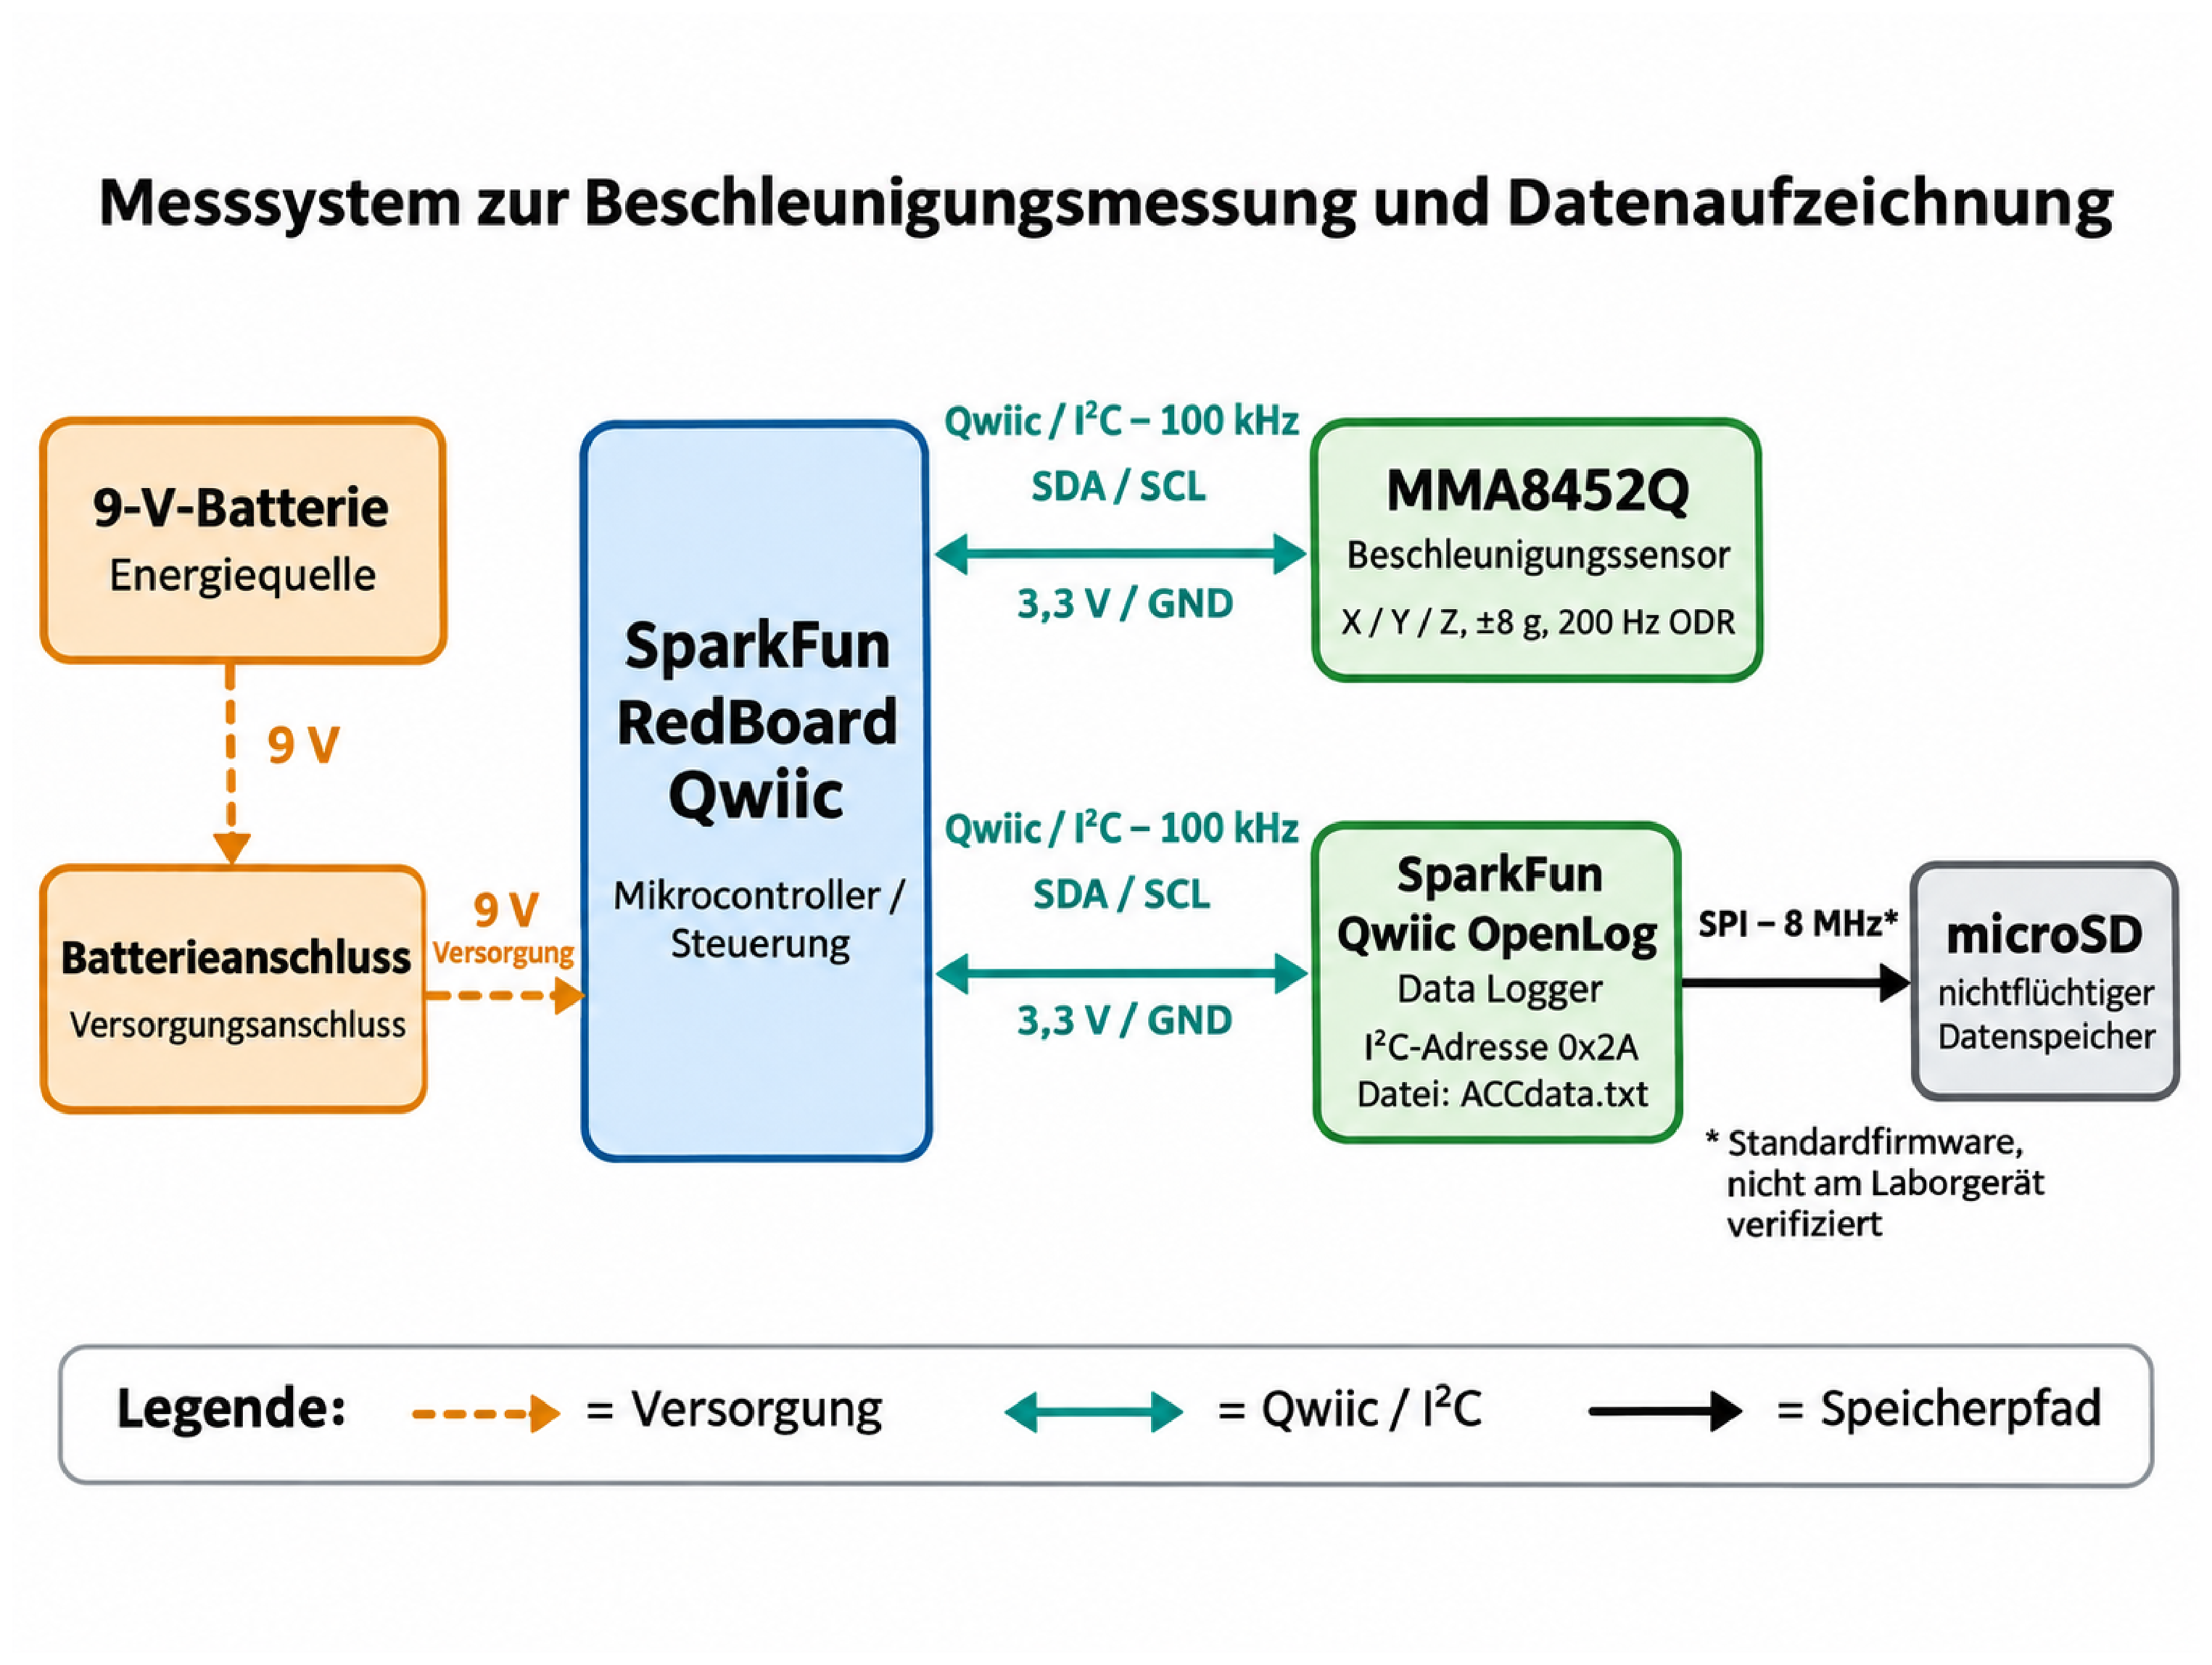
\includegraphics[width=\linewidth,keepaspectratio]{abbildungen/messsystem_aufgabe1_neu.eps}
    \caption{Blockschaltbild des Messsystems zur Beschleunigungsmessung und
    Datenaufzeichnung (eigene Darstellung; SPI-Takt nach Standardfirmware).}
    \label{fig:messsystem}
\end{figure}

\textbf{9-V-Batterie:}
Die Batterie stellt die externe elektrische Energie f\"ur das Messsystem bereit.

\textbf{Batterieanschluss:}
Der Anschluss verbindet die 9-V-Batterie mit dem vorgesehenen
Versorgungseingang des SparkFun RedBoards.

\textbf{SparkFun RedBoard Qwiic:}
Das RedBoard steuert die Messung, liest die Beschleunigungswerte des Sensors
aus und \"ubermittelt sie an den Data Logger. Die Kommunikation mit beiden
Qwiic-Modulen erfolgt \"uber I$^2$C (SDA/SCL) mit einem Standardtakt von
100\,kHz; die Module werden \"uber den Qwiic-Anschluss mit 3,3\,V und GND versorgt.

\textbf{MMA8452Q-Beschleunigungssensor:}
Der Sensor erfasst die Beschleunigungen entlang der drei Achsen X, Y und Z.
Im bereitgestellten Arduino-Programm zur Datenaufzeichnung mit dem Qwiic
OpenLog sind ein Messbereich von $\pm 8\,\mathrm{g}$ und eine Sensordatenrate
(ODR) von $200\,\mathrm{Hz}$ eingestellt.

\textbf{SparkFun Qwiic OpenLog:}
Der Data Logger empf\"angt die vom RedBoard \"ubertragenen Messwerte \"uber
den I$^2$C-Bus (Standardadresse \texttt{0x2A}) und zeichnet sie in der Datei
\texttt{ACCdata.txt} auf der microSD-Karte auf.

\textbf{microSD-Karte:}
Die Speicherkarte dient als nichtfl\"uchtiger Datenspeicher und ist im
OpenLog eingesteckt. Ihre interne Anbindung erfolgt \"uber SPI; die in der
Grafik genannten 8\,MHz beziehen sich auf die Standardfirmware und wurden
am Laborger\"at nicht eigens verifiziert.
